% (c) 2015 Daniele Zambelli daniele.zambelli@gmail.com

% % \vspace{-2ex}% (c) 2012 Dimitrios Vrettos - d.vrettos@gmail.com
  \begin{center}
    \begin{hieroglyph}{\leavevmode \loneSign{\Aca GM/43/}\HinterSignsSpace
\loneSign{\Aca GM/43/}\HinterSignsSpace
\loneSign{\Aca GM/43/}\HinterSignsSpace
\Cadrat{\CadratLineI{\Aca GV/32/\hfill\Aca GV/32/\hfill\Aca GV/32/}\CadratLine{\Aca GV/32/\hfill\Aca GV/32/\hfill\Aca GV/32/}}\HinterSignsSpace
\Cadrat{\CadratLineI{{\Hsmaller\Hsmaller\Aca GV/51/}\hfill{\Hsmaller\Hsmaller\Aca GV/51/}\hfill{\Hsmaller\Hsmaller\Aca GV/51/}}\CadratLine{\Aca GV/51/\hfill\Aca GV/51/\hfill\Aca GV/51/\hfill\Aca GV/51/}}\HinterSignsSpace
\loneSign{\Aca GZ/32/}\HinterSignsSpace
\loneSign{\Aca GZ/32/}\HinterSignsSpace
\loneSign{\Aca GZ/32/}}\end{hieroglyph}
  \end{center}\vspace{-2ex}
% \begin{inaccessibleblock}
% [Immagine di una porzione dell'insieme di Mandelbrot.]
% \vspace{-2ex}
% \begin{center} 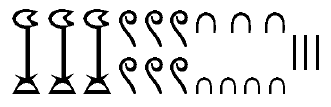
\includegraphics[scale=0.25]{img/hiero3673.png} \end{center}
% \vspace{-2ex}
% \end{inaccessibleblock}

\chapter{Dai Naturali agli Iperreali}

\section{Dai numeri naturali ai numeri irrazionali}
\label{sec:01_introduzione}

Riprendiamo i diversi insiemi numerici che abbiamo imparato a conoscerete
mettendo in evidenza il loro ruolo come modelli per risolvere alcune classi di 
problemi e le loro caratteristiche.

\subsection{I numeri naturali $\N$}
\label{subsec:insnum_naturali}

I primi numeri che abbiamo incontrato sono i numeri naturali. Sono quelli che 
permettono di contare oggetti. Se sul banco ho un quaderno, una penna e un 
libro posso dire che ci sono~3 oggetti. Si può capire come il numero Zero abbia 
avuto difficoltà a farsi accettare come numero: serve per contare un gruppo di 
oggetti dove non c'è niente da contare. Ma ora abbiamo capito che è molto 
comodo considerare lo zero come un numero.
Questi numeri sono chiamati numeri \emph{naturali} 
e l'insieme di questi numeri viene indicato con~$\N$.

Nei numeri naturali sono definite l'addizione, la moltiplicazione che sono 
sempre possibili. In queste due \emph{strutture} $\tonda{\N, +}$ e 
$\tonda{\N, \times}$ valgono le proprietà: associativa, commutativa e 
l'esistenza dell'elemento neutro.

Nei numeri naturali è definita anche la \emph{potenza} ma questa operazione non 
è definita quando sia la base sia l'esponente sono uguali a zero.

Oltre a queste, sono definite anche le loro operazioni inverse: la sottrazione, 
la divisione e la radice, queste non sono definite per ogni coppia di numeri.

D'altra parte se su un tavolo ho~5 oggetti posso toglierne~3 e ne restano~2:
\[5-3=2\]

Ma se sul tavolo ho~3 oggetti non ha senso cercare di toglierne~5!

\subsection{I numeri interi $\Z$}
\label{subsec:insnum_interi}

I numeri possono però essere utilizzati anche come modelli di altre situazioni. 
Supponiamo di avere la sequenza di oggetti e di voler riferirmi ad ognuno con 
un numero che equivale al suo indirizzo o indice. In certi casi potrei cercare 
il primo elemento della sequenza e chiamarlo zero, quello che viene dopo lo 
chiamo uno e così via. Ma se ci trovassimo a lavorare principalmente con gli 
elementi compresi tra il 273° elemento e il 310° elemento, questo modo di fare 
sarebbe piuttosto scomodo. Molto più semplice è mettersi d'accordo di chiamare 
zero il 273° elemento e partire da lì a contarli. Ora i numeri che dovremo 
usare saranno quelli compresi tra~0 e~37. Ci sono inoltre delle situazioni in 
cui è difficile, o impossibile, determinare un \emph{primo} elemento della 
sequenza e anche in questo caso ci si può mettere d'accordo di assegnare ad un 
preciso elemento della sequenza il valore zero.

E chiaro che lo \emph{zero} non sarà il \emph{primo} elemento della sequenza, 
ma un valore all'interno della sequenza. Quindi è possibile muoversi sia sopra 
lo zero, sia sotto lo zero. I numeri dallo zero in poi posso corrispondere ai 
naturali ma dobbiamo aggiungere altri infiniti numeri, tutti quelli prima dello 
zero. Per non inventare dei nomi completamente nuovi per questi nuovi numeri, 
sono stati aggiunti semplicemente due segni:~$+$ per i numeri dopo lo zero 
e~$-$ per i numeri prima dello zero. 
Questi nuovi numeri sono chiamati numeri \emph{interi} 
e l'insieme di questi numeri viene indicato con~$\Z$.

In questa situazione l'addizione può essere vista come muoversi nel verso di 
crescita dei numeri e la sottrazione come muoversi nel verso della decrescita 
dei numeri. Dato che lo zero è un elemento convenzionale non c'è nessun 
problema a togliere~5 da~3 semplicemente si arriverà nella posizione~2 prima 
dello zero detta anche~$-2$.

In questo insieme di numeri è sempre definita anche la sottrazione, anzi la 
sottrazione diventa semplicemente un caso particolare di addizione.

I numeri interi permettono di risolvere sempre equazioni del tipo:
\[x+a=0\]

Anche questi numeri però non riescono a realizzare un modello in certe 
situazioni che invece nella pratica si possono risolvere facilmente con un po' 
di creatività. Ad esempio come possiamo dividere~3 uova, in parti uguali, tra~4 
persone?

\subsection{I numeri razionali $\Q$}
\label{subsec:insnum_razionali}

Con le tre uova faccio una frittata che divido facilmente in~4 parti uguali. 
Possiamo costruire dei numeri che permettano di calcolare sempre il quoziente 
esatto di due numeri naturali anche quando la divisione tra i due dà un resto 
diverso da zero. Questi nuovi numeri sono chiamati numeri \emph{razionali} 
e l'insieme di questi numeri viene indicato con~$\Q$.

Mentre nei naturali e negli interi ad ogni numero corrisponde un \emph{nome} 
ben preciso, nei razionali lo stesso numero può essere indicato con molti nomi 
diversi. Ad esempio il numero che si ottiene dividendo~1 in due parti uguali 
può essere indicato in in uno di questi modi:
\[\frac{1}{2}=\frac{3}{6}=\frac{45}{90}=\frac{132}{264}=0,5\]

Ogni numero razionale può essere rappresentato con un numero con la virgola o 
con una qualunque delle infinite frazioni equivalenti.

Con i numeri razionali si può sempre calcolare il risultato della divisione tra 
due numeri (naturali, interi o razionali) tranne il caso particolare in cui il 
divisore sia uguale a zero. 
In questo caso la divisione non può essere eseguita.

I numeri razionali permettono di risolvere sempre equazioni del tipo:
\[ax+b=0\]

I razionali hanno una caratteristica particolare che non avevano né i naturali 
né gli interi: formano un insieme \emph{denso} cioè tra due numeri razionali, 
per quanto vicini, se ne può trovare sempre almeno un altro.

Ma ci sono ancora situazioni in cui i numeri razionali non permettono di 
risolvere problemi relativamente semplici da risolvere praticamente. 
Ad esempio è stato dimostrato (già qualche millennio fa) che se il lato di un 
quadrato è un numero razionale allora la sua diagonale non lo è. 

\subsection{I numeri reali $\R$}
\label{subsec:insnum_reali}

Se prendiamo un quadrato di lato~1, la sua diagonale, per il teorema di 
Pitagora, risulta lunga~$\sqrt{2}$. 
La radice di due è quel numero che elevato alla seconda dà come risultato~2.
Ebbene, è stato dimostrato che nessun numero razionale moltiplicato per se 
stesso dà come risultato~2. Quindi, o dà un numero più piccolo o un numero più 
grande.

Possiamo quindi costruire due sottoinsiemi dell'insieme $\Z$ in modo da mettere 
in uno tutti i numeri minori di un certo valore e nell'altro tutti i numeri 
maggiori o uguali a quel valore. Nel caso della radice di~2:

\begin{center}
 \begin{tabular}{ll}
\toprule
Valore per difetto di $\sqrt{2}$ &Valore per eccesso di $\sqrt{2}$ \\
\midrule
1& 2\\
1,4& 1,5 \\
1,41& 1,42\\
1,414& 1,415\\
1,4142& 1,4143\\
\ldots& \ldots\\
\bottomrule
\end{tabular}
\end{center}

Due sottoinsiemi costruiti in questo modo si chiamano classi contigue di 
numeri razionali. Due classi contigue di numeri razionali definiscono un numero 
\emph{reale} $\R$. Dato un \emph{numero qualsiasi} possiamo sempre realizzare 
due classi contigue di numeri razionali. Se questo \emph{numero qualsiasi} 
appartiene al secondo sottoinsieme è, evidentemente un numero razionale, se non 
appartiene ai due sottoinsiemi è un numero irrazionale. Ognuna di queste 
partizioni, dette anche sezioni di Dedekind, può essere considerata come un
numero, cioè è possibile costruire un ordine tra le sezioni, sommarle, 
moltiplicarle, \dots

I numeri reali formano un insieme \emph{ordinato}, \emph{denso} ma anche 
\emph{completo} cioè il numero individuato da una qualunque sezione di Dedekind 
è un numero reale.
Questo permette di far corrispondere ad ogni punto della \emph{retta reale}un 
numero \emph{reale} e viceversa 
ad ogni numero \emph{reale} un punto della \emph{retta reale}. 

Bene l'insieme dei numeri reali permette di risolvere tutti i problemi che 
possiamo incontrare? 

\begin{center} \emph{Per fortuna no!} \end{center} 

Ci sono tipi di problemi che non possono essere risolti con i numeri reali.
Ad esempio calcolare la radice quadrata di numeri negativi. Anche questo 
all'apparenza è un problema del tutto assurdo: calcolare la radice quadrata di 
un numero equivale a trovare la lunghezza del lato di un quadrato di cui si 
conosce l'area. Ora trovare un quadrato con area piccola si può fare, anche con 
area nulla, impegnandosi un po', ma trovare un quadrato con area negativa 
è proprio impossibile. Ma come abbiamo visto per i naturali ci possono essere 
fenomeni nei quali hanno senso operazioni che in altri sistemi sono insensate.

\subsection{I numeri complessi $\C$}
\label{subsec:insnum_complessi}

Si può ampliare l'insieme dei numeri reali aggiungendo i numeri che sono le 
radici di tutti i numeri anche di quelli negativi. Per fare ciò si devono 
aggiungere molti altri numeri (infiniti) tutti questi nuovi numeri sono stati 
chiamati numeri \emph{immaginari} che combinati con i numeri reali formano 
l'insieme dei numeri \emph{complessi} insieme che viene indicato con $\C$.

\begin{wrapfloat}{figure}{r}{0pt}
\begin{inaccessibleblock}
[Immagine di una porzione dell'insieme di Mandelbrot.]

\includegraphics[scale=0.30]{img/fractal.jpg}
\end{inaccessibleblock}
\caption{Porzione dell'insieme di Mandelbrot.}
\label{fig:mandelbrot}
\end{wrapfloat}

Questi numeri hanno molte applicazioni tecniche, ma risultano anche 
affascinanti da un punto di vista estetico. La ripetizione di un paio di 
calcoli aritmetici tra numeri complessi produce il sorprendente insieme di 
Mandelbrot.

Ma dato che l'insieme dei reali oltre che essere un campo ordinato è anche 
completo, non è possibile aggiungere elementi ai reali senza perdere qualche 
proprietà dell'insieme numerico. Nel caso dei complessi l'insieme ottenuto non 
è totalmente ordinato.

% \vspace{24pt}

\section{I numeri iperreali $\IR$}
\label{sec:insnum_iperreali}

In questa sezione vedremo altri insiemi numerici che permettono di 
modellizzare e risolvere altre classi di problemi.

\subsection{Il problema della velocità}
\label{subsec:insnum_velocita}

Alla fine del 1600 Newton e Leibniz studiavano problemi legati alla meccanica. 
Una delle grandezze alla base della meccanica è la \emph{velocità}. Ma cosa è 
la velocità? Se l'oggetto A percorre più strada dell'oggetto B possiamo dire 
che A è più veloce di B? No, non basta misurare lo spazio percorso da un 
oggetto per calcolare la sua velocità, bisogna anche misurare il tempo 
impiegato a percorrere quello spazio. Possiamo dire che:
\[velocità = \frac{spazio percorso}{tempo impiegato}\]

La grandezza calcolata in questo modo è \emph{la velocità media} dell'oggetto, 
ma in ogni istante del percorso l'oggetto ha una propria velocità. Come faccio 
a calcolarla? Posso misurare lo spazio percorso in un tempo molto piccolo, in 
questo modo avrò una velocità media tenuta in un percorso molto breve. Più 
restringo l'intervallo di tempo, più la velocità media si avvicina alla 
velocità istantanea \dots ma resta sempre una velocità media. 

Per trovare la velocità istantanea dovrei dividere lo spazio percorso per un 
tempo (positivo) più piccolo di qualunque numero. Ma l'unico numero 
positivo più piccolo di qualunque numero è lo zero, ma la divisione per 
zero non è definita. I numeri reali non ci permettono di calcolare una 
grandezza così semplice e evidente come la velocità di un oggetto in un dato 
istante.

Servirebbe un insieme numerico con dei numeri positivi più piccoli di un 
qualsiasi altro numero positivo, ma diversi da zero! Magari questi numeri ci 
sono già nell'insieme dei reali che, come abbiamo visto, è un insieme completo.

\subsection{Il postulato di Eudosso-Archimede}
\label{subsec:insnum_eudossoarchimede}

Proviamo a fare un \emph{semplice} esperimento mentale. Prendo un foglio di 
carta e lo piego su se stesso un po' di volte. Che spessore raggiungo?
Per semplificarci i calcoli supponiamo che il foglio di carta abbia lo spessore 
di $0,1mm = 0,0001m = 10^{-4}m$. 
Che spessore otterrò piegando il foglio su se stesso~64 volte?

Il calcolo è abbastanza semplice:

\begin{center}
 \begin{tabular}{ccc}
\toprule
Numero piegature & spessore ottenuto & in metri\\
\midrule
0 & 1 & $10^{-4}$\\
1 & 2 & $10^{-4}$\\
2 & 4 & $10^{-4}$\\
3 & 8 & $10^{-4}$\\
4 & 16 & $10^{-3}$\\
5 & 32 & $10^{-3}$\\
6 & 64 & $10^{-3}$\\
7 & 128 & $10^{-2}$\\
\ldots& \ldots\\
n & $2^n$ & \ldots\\
\bottomrule
\end{tabular}
\end{center}

Quindi piegando il foglio 64 volte ottengo uno spessore che è $2^{64}$ volte lo 
spessore di partenza quindi basta calcolare:

\[2^{64} = 18.446.744.073.709.551.616\]
che convertito in metri dà: $1.844.674.407.370.955m$ circa che è uno spessore 
considerevole, quasi duemila volte la distanza Terra-Sole:~$149.600.000.000m$.

Si fa risalire ai matematici Eudosso e Archimede l'osservazione che per quanto 
piccolo si prenda un numero (lo spessore di un foglio di carta), basta 
moltiplicarlo per un numero sufficientemente grande~($2^{64}$) per farlo 
diventare maggiore di qualsiasi numero (la distanza Terra-Sole).

Vale anche il contrario: per quanto grande sia un numero posso dividerlo per un 
numero abbastanza grande da farlo diventare più piccolo di un qualunque numero.

Ma questa osservazione di Eudosso-Archimede non è un teorema, non è 
un'osservazione dimostrata, è un postulato, un accordo fatto tra matematici che 
può essere utile in moltissimi casi e che vale per tutti gli insiemi numerici 
visti fin'ora. Ma cosa succede se ci accordiamo che non valga il postulato di 
Eudosso-Archimede?

\subsection{Insiemi non archimedei}
\label{subsec:insnum_nonarchimedei}

Vogliamo costruire un insieme numerico non archimedeo. Per farlo aggiungiamo 
all'insieme dei numeri reali un nuovo numero (non reale):

\[\varepsilon > 0 \text{ tale che } 
\varepsilon < \frac{1}{n} \text{ per qualunque } n \in \N\]

tradotto in simboli:

\[\varepsilon > 0 \quad | \quad \varepsilon < \frac{1}{n} \quad \forall n \in 
\N\]

Ovviamente un tale numero non può essere un numero reale e un numero siffatto 
lo chiameremo un \emph{infinitesimo} e lo indicheremo con $\epsilon$ 
(o con un'altra lettera minuscola dell'alfabeto greco).

La prima conseguenza all'introduzione di un infinitesimo è che allora ce ne 
sono infiniti! Infatti anche la metà di un infinitesimo è un infinitesimo e 
anche il suo doppio o un suo sottomultiplo o un suo multiplo.

Altra conseguenza dell'aggiunta di un elemento infinitesimo all'insieme dei 
reali è che se esiste un numero maggiore di zero più piccolo di tutti gli altri 
numeri allora esiste anche un numero maggiore di qualunque altro numero:

\[\text{se} \quad \varepsilon < \frac{1}{n} \quad \forall n \in \N 
\quad \text{allora} \quad \frac{1}{\varepsilon} > n \quad \forall n 
\in \N\]

Quindi se aggiungiamo all'insieme dei reali un numero infinitesimo e possiamo 
fare le solite operazioni sull'infinitesimo, allora in quell'insieme avremo un 
numero infinito di infinitesimi e un numero infinito di infiniti.

Chiamiamo \emph{iperreali} l'insieme numerico così ottenuto e lo indichiamo con 
il simbolo:~$\IR$.

\subsection{Tipi di Iperreali}
\label{subsec:insnum_nonarchimedei}

Abbiamo visto che l'introduzione di un elemento nuovo, quasi inesistente, ha 
reso piuttosto affollato il nuovo insieme numerico. Cerchiamo di fare un po' 
di ordine. L'insieme degli Iperreali contiene:

\begin{itemize} [noitemsep]
 \item i numeri reali che d'ora in poi verranno chiamati anche numeri 
\emph{standard}, tra questi c'è anche lo zero;
 \item gli infinitesimi, lo zero è l'unico infinitesimo che è anche un numero 
reale;
 \item i numeri non reali che non sono né infinitesimi né infiniti;
 \item gli infiniti, nessun infinito ha una corrispondenza con i numeri reali.
\end{itemize}

Possiamo veder questo insieme anche come formato dai seguenti elementi:

\begin{description} [noitemsep]
 \item \textbf{zero}
 è un infinitesimo ed è un numero standard;
 \item \textbf{infinitesimi non nulli}
 tutti gli infinitesimi diversi da zero;
 \item \textbf{finiti}
 tutti quei numeri che sono, in valore assoluto, minori di un numero reale;
 \item \textbf{finiti non infinitesimi}
 tutti quei numeri che sono in valore assoluto compresi tra due numeri reali 
 diversi da zero;
 \item \textbf{infiniti}
 tutti quei numeri che sono maggiori di qualsiasi numero reale

\end{description}
 
Per semplificare la scrittura (e complicare la lettura) adotteremo delle sigle 
e delle convenzioni per indicare questi diversi tipi di numeri:

\begin{center}
\begin{tabular}{ccc}\toprule
tipo & sigla & simboli\\\midrule
zero &  & 0\\
infinitesimo & \emph{i} & \\
infinitesimo non nullo & \emph{inn} & $\alpha, \beta, \gamma, \delta, \dots$\\
finito non infinitesimo& \emph{fni} & a, b, c, d, ...\\
finito & \emph{f} & a, b, c, d, ...\\
infinito & \emph{I} & A, B, C\\
qualsiasi &  & x, y, z, \ldots\\\bottomrule
\end{tabular}
\label{tab:insnum_tipi}
\end{center}

\subsection{Iperreali finiti e parte standard}
\label{subsec:insnum_partestandard}

Gli Iperreali finiti sono quei numeri che sono compresi tra due numeri Reali:

\begin{definizione}
 Il numero Iperreale $x$ è compreso tra due numeri Reali allora $x$ è un 
Iperreale finito:

\[\text{Se } x \in \IR \wedge a, b \in \R \wedge 
  a < x < b \text{ allora } x \text{ è un Iperreale finito.}\]
\end{definizione}

Ogni numero finito può essere visto come la somma di un numero reale più un 
Infinitesimo: se $x$ è finito allora $x = a + \epsilon$. Un numero Iperreale 
finito non può essere infinitamente vicino a due numeri reali diversi quindi 
esiste un solo numeri Reale infinitamente vicino ad un numero Iperreale. 
Questo numero reale si chiama \emph{parte standard} del numeri Iperreale.

\begin{definizione}
 La parte standard di un numero Iperreale finito è il l'unico numero Reale 
infinitamente vicino:

\[\text{Se } x \in \IR \wedge x= a+\epsilon \text{ allora } 
a= \st(x) \text{ (st = parte standard).}\]
\end{definizione}


\subsection{Retta Iperreale e strumenti ottici}
\label{subsec:insnum_retta}

In un paragrafo precedente abbiamo visto che si può accettare un postulato che 
dice che ad ogni numero reale corrisponde un punto della retta e ad ogni 
punto della retta corrisponde un numero reale. 
Questa affermazione non è un teorema dimostrato, è un postulato. Visto che 
abbiamo già fatto saltare il postulato di Eudosso-Archimede, cambiamo anche 
questo postulato e lo riformuliamo così:

\begin{postulato}
Ad ogni numero Iperreale corrisponde un punto della retta (iperreale) e ad ogni 
punto della retta (iperreale) corrisponde un numero Iperreale.
\end{postulato}

Oppure:

\begin{postulato}
C'è una corrispondenza biunivoca tra i numeri Iperreali e 
i punti della retta (iperreale).
\end{postulato}

Con i numeri reali abbiamo una certa abitudine a rappresentare numeri.
Per rappresentare i numeri Iperreali dobbiamo procurarci degli strumenti 
particolari: \emph{microscopi}, \emph{telescopi}, \emph{grandangoli}.

Diamo una sbirciata al loro manuale di istruzioni.

\subsubsection{Microscopi}
\label{subsec:insnum_microscopio}

Il microscopio permette di ingrandire una porzione di retta. 
Un microscopio permette di visualizzare i seguenti numeri:

\begin{multicols}{4}
\begin{itemize}
 \item $+5,004$
 \item $-3,000002$
 \item $2-\epsilon$
 \item $-4+\delta$
\end{itemize}
\end{multicols}

Si può osservare come ci siano microscopi ``standard'' che ingrandiscono un 
numero \emph{naturale} di volte e microscopi ``non standard'' che ingrandiscono 
infinite volte.

\subsubsection{Telescopi}
\label{subsec:insnum_microscopio}

Il telescopio permette di avvicinare una porzione di retta senza cambiare la 
sua scala. 
Con un telescopio possiamo visualizzare i seguenti numeri:

\begin{multicols}{4}
\begin{itemize}
 \item $+127034$
 \item $-3600$
 \item $A+3$
 \item $-B+2$
\end{itemize}
\end{multicols}

Anche per i telescopi, i modelli più moderni offrono la possibilità di operare 
ingrandimenti ``standard'' o ``non standard'' a piacere.

\subsubsection{Grandangoli (Zoom)}
\label{subsec:insnum_microscopio}

Il Grandangolo permette di cambiare la scala della visualizzazione della retta, 
in questo modo possiamo far rientrare nel campo visivo anche numeri molto 
lontani.
Possiamo usare uno zoom per visualizzare i seguenti numeri:

\begin{multicols}{4}
\begin{itemize}
 \item $500$
 \item $-3000$
 \item $2A$
 \item $3B$
\end{itemize}
\end{multicols}

Anche per questi strumenti utilizzeremo versioni che permettono zoomate 
``standard'' e ``non standard''.

\subsection{Operazioni}
\label{subsec:insnum_operazioni}

Vediamo di seguito alcune regole relative alle operazioni 
che valgono nei numeri Iperreali.

\subsubsection{Addizione}
\label{subsec:insnum_addizione}

Alcune osservazioni:

\begin{enumerate} [noitemsep]
 \item Le regole relative all'addizione valgono anche per la sottrazione, se 
uno degli addendi è negativo. 
 \item Zero è l'elemento neutro dell'addizione nei Reali e continua ad esserlo 
anche negli Iperreali: $x+0=0+x=x$.
 \item Un infinitesimo più un altro infinitesimo dà per risultato un 
infinitesimo: $\alpha+\beta=\gamma$.
 \item Un infinitesimo non nullo più un altro infinitesimo non nullo può dare 
per risultato anche zero: \dots
 \item Un finito più un infinitesimo dà come risultato un finito.
 \item Un finito più un finito dà come risultato un finito.
 \item Un finito più un finito può dare come risultato un infinitesimo.
%  \item Un infinito più un infinitesimo dà come risultato un infinito.
 \item Un infinito più un finito dà come risultato un infinito.
 \item Un infinito più un infinito può dare come risultato zero, un 
infinitesimo, un finito non infinitesimo, un finito, un infinito.
\end{enumerate}

Nel precedente elenco abbiamo visto che alcune addizioni danno un risultato 
che dipende solo dai tipi degli operandi, altre operazioni danno dei risultati 
che dipendono dal valore degli operandi. Possiamo costruire una tabella che 
organizza le precedenti osservazioni.

\begin{center}
\renewcommand{\arraystretch}{.0}
\scalebox{0.8}{
\begin{tabular}{p{.7cm}|p{.7cm}|p{.7cm}|p{.7cm}|p{.7cm}|p{.7cm}|}
\centra{$+$} & \centra{0} & \centra{inn} & \centra{fni} & \centra{I} \\\hline
\centra{0} & \centra{0} & \centra{inn}& \centra{fni} & \centra{I} \\\hline
\centra{inn} & \centra{inn} & \centra{i}& \centra{fni} & \centra{I} \\\hline
\centra{fni} & \centra{fni} & \centra{fni}& \centra{f} & \centra{I} \\\hline
\centra{I} & \centra{I} & \centra{I}& \centra{I} & \centra{?} \\\hline
\end{tabular}}
\end{center}

\subsubsection{Moltiplicazione}
\label{subsec:insnum_moltiplicazione}

\noindent \begin{minipage}{.5\textwidth}
Alcune osservazioni:
\begin{enumerate} [noitemsep]
 \item Zero è l'elemento assorbente: il prodotto di un iperreale per zero
dà come risultato zero: $x \cdot 0=0 \cdot x=0$.
 \item Uno è l'elemento neutro della moltiplicazione nei Reali e continua ad 
esserlo anche negli Iperreali: $x \cdot 1=1 \cdot x=x$.
 \item Un infinitesimo per un altro infinitesimo dà per risultato un 
infinitesimo: $\alpha \cdot \beta=\gamma$.
 \item Un infinitesimo non nullo per un altro infinitesimo non nullo da 
per risultato un infinitesimo non nullo.
 \item \dots
%  \item Un finito per un infinitesimo dà come risultato un finito.
%  \item Un finito per un finito dà come risultato un finito.
%  \item Un finito per un finito può dare come risultato un infinitesimo.
% %  \item Un infinito per un infinitesimo dà come risultato un infinito.
%  \item Un infinito per un finito dà come risultato un infinito.
%  \item Un infinito per un infinito può dare come risultato zero, un 
% infinitesimo, un finito non infinitesimo, un finito, un infinito.
\end{enumerate}
\end{minipage}
\hfill
\begin{minipage}{.45\textwidth}
E la tabella corrispondente:
\begin{center}
\renewcommand{\arraystretch}{.0}
\scalebox{0.8}{
\begin{tabular}{p{.7cm}|p{.7cm}|p{.7cm}|p{.7cm}|p{.7cm}|p{.7cm}|}
\centra{$\times$} & \centra{0} & \centra{1} & 
\centra{inn} & \centra{fni} & \centra{I} \\\hline
\centra{0} & \centra{0} & \centra{0} & 
\centra{0}& \centra{0} & \centra{0} \\\hline
\centra{1} & \centra{0} & \centra{1} & 
\centra{inn} & \centra{fni} & \centra{I} \\\hline
\centra{inn} & \centra{0} & \centra{inn} & 
\centra{inn}& \centra{inn} & \centra{?} \\\hline
\centra{fni} & \centra{0} & \centra{fni} & 
\centra{inn}& \centra{fni} & \centra{I} \\\hline
\centra{I} & \centra{0} & \centra{I} & 
\centra{?}& \centra{I} & \centra{I} \\\hline
\end{tabular}}
\end{center}
\vspace{2mm}
\end{minipage}

\subsubsection{Divisione}
\label{subsec:insnum_divisione}


\noindent \begin{minipage}{.5\textwidth}
Alcune osservazioni:
\begin{enumerate} [noitemsep]
 \item Anche negli Iperreali la divisione per zero non è definita.
 \item Uno può essere visto come un elemento neutro solo destro: $x \div 1=x$.
 \item Per cercare i risultati possiamo rifarci alla definizione di quoziente.
 \item \dots
%  \item Un infinitesimo per un altro infinitesimo dà per risultato un 
% infinitesimo: $\alpha \cdot \beta=\gamma$.
%  \item Un infinitesimo non nullo per un altro infinitesimo non nullo da 
% per risultato un infinitesimo non nullo.
%  \item Un finito per un infinitesimo dà come risultato un finito.
%  \item Un finito per un finito dà come risultato un finito.
%  \item Un finito per un finito può dare come risultato un infinitesimo.
% %  \item Un infinito per un infinitesimo dà come risultato un infinito.
%  \item Un infinito per un finito dà come risultato un infinito.
%  \item Un infinito per un infinito può dare come risultato zero, un 
% infinitesimo, un finito non infinitesimo, un finito, un infinito;
\end{enumerate}
\vspace{20mm}
\end{minipage}
\hfill
\begin{minipage}{.45\textwidth}
E la tabella corrispondente:
\begin{center}
\renewcommand{\arraystretch}{.0}
\scalebox{0.8}{
\begin{tabular}{p{.7cm}|p{.7cm}|p{.7cm}|p{.7cm}|p{.7cm}|p{.7cm}|}
% \begin{tabular}{c|c|c|c|c|c|}
\centra{$\div$} & \centra{0} & \centra{1} & 
\centra{inn} & \centra{fni} & \centra{I} \\\hline
\centra{0} &  & \centra{0} & 
\centra{0}& \centra{0} & \centra{0} \\\hline
\centra{1} &  & \centra{1} & 
\centra{I} & \centra{fni} & \centra{inn} \\\hline
\centra{inn} &  & \centra{inn} & 
\centra{?}& \centra{inn} & \centra{inn} \\\hline
\centra{fni} &  & \centra{fni} & 
\centra{I}& \centra{fni} & \centra{inn} \\\hline
\centra{I} &  & \centra{I} & 
\centra{I}& \centra{I} & \centra{?} \\\hline
\end{tabular}}
\end{center}
\end{minipage}

\subsubsection{Reciproco}
\label{subsec:insnum_reciproco}

\noindent \begin{minipage}{.5\textwidth}
Alcune osservazioni:
\begin{enumerate} [noitemsep]
 \item Dalla tabella precedente si può estrarre la riga corrispondente a~1
e si ottiene la tabella del reciproco.
 \item Una volta convinti della regola del reciproco, si può ricavare la 
tabella della divisione attraverso la 
regola:~$x \div y = x \times \tonda{\frac{1}{y}}$.
\end{enumerate}
\end{minipage}
\hfill
\begin{minipage}{.45\textwidth}
E la tabella corrispondente:
\begin{center}
\renewcommand{\arraystretch}{.0}
\scalebox{0.8}{
\begin{tabular}{p{1.7cm}|p{.7cm}|p{.7cm}|p{.7cm}|p{.7cm}|p{.7cm}|}
\centra{numero} & \centra{0} & \centra{1} & 
\centra{inn} & \centra{fni} & \centra{I} \\\hline
\centra{reciproco} &  & \centra{1} & 
\centra{I} & \centra{fni} & \centra{inn} %\\\hline
\end{tabular}}
\end{center}
\vspace{11mm}
\end{minipage}

\begin{osservazione}
Non ci sono regole immediate per le seguenti operazioni:
\begin{multicols}{4}
\begin{itemize} [nosep]
 \item \(\dfrac{\epsilon}{\delta}\)
 \item \(\dfrac{A}{B}\)
 \item \(A \cdot \epsilon\)
 \item \(A + B\)
\end{itemize}
\end{multicols}
In questi casi il tipo di risultato dipende dall'effettivo valore degli 
operandi. Ad esempio, nel caso del quoziente tra due infinitesimi possiamo 
trovarci nelle seguenti situazioni:
\begin{multicols}{3}
\begin{itemize} [nosep]
 \item \(\dfrac{\epsilon^2}{\epsilon} = \epsilon\) \quad (i)
 \item \(\dfrac{2\epsilon}{\epsilon} = 2\) \quad (fni)
 \item \(\dfrac{\epsilon}{\epsilon^2} = \frac{1}{\epsilon}\) \quad (I)
\end{itemize}
\end{multicols}
\end{osservazione}

Possiamo ora esercitarci nel calcolo con questi nuovi numeri. 
Continuiamo ad utilizzare la convenzione di indicare gli 
infinitesimi con lettere greche minuscole
($\alpha,~\beta,~\gamma,~\delta,~\epsilon,~\dots$), 
i finiti non infinitesimi con lettere latine minuscole 
($a,~b,~c~,~\dots,~m,~n,~\dots$) 
e gli infiniti con lettere latine maiuscole 
($A,~B,~C~,~\dots,~M,~N,~\dots$).

\begin{exrig}
Semplifichiamo le seguenti espressioni scrivendo il tipo di risultato ottenuto.

 \begin{esempio}
  $3\epsilon +5 +6M -2\epsilon +7 -2M = 4M +12 +\epsilon \quad (tipo=I)$
 \end{esempio}

\begin{osservazione}
Quando il risultato è la somma di più elementi, li scriviamo, ordinandoli dal 
più grande, in valore assoluto, al più piccolo.
%  Quando possibile scriviamo un risultato composto da più elementi scrivendoli 
% dal più grande, in valore assoluto, al più piccolo.
\end{osservazione}

 \begin{esempio}
\(7 +8M -5\epsilon  -4 +3\epsilon-2N = 8M -2N +3 -2\epsilon\)
\quad (tipo non definito)
 \end{esempio}
 
 \begin{esempio}
\(\tonda{3M +2\epsilon} \tonda{3M -2\epsilon} = 9M -4\epsilon\)
\quad (tipo=I)
 \end{esempio}
 
 \begin{esempio}
\(\tonda{M +3} \tonda{M -3} - \tonda{M+2}^2 +4\tonda{M +3}=\)

\(=M^2 -9 -M^2 -4M -4 +4M +12 = -1\)
\quad (tipo=fni)
 \end{esempio}
 
 \begin{esempio}
\(10a -\tonda{A +1}^2 -3a +2\tonda{a+2\alpha} +A^2 +6\tonda{b -3\alpha} +2A= \)

\(=10a -A^2 -2A -1 -3a +2a+4\alpha +A^2 +6b -18\alpha +2A = 9a +6b -14\alpha\) 
\quad (tipo=fni)
 \end{esempio}
\end{exrig}

% \subsection{Espressioni}
% \label{subsec:insnum_espressioni}

\subsection{Confronto}
\label{subsec:insnum_confronto}

L'insieme dei numeri Reali ha un ordinamento completo, se $a$ e $b$ sono due 
numeri reali qualunque è sempre valida una e una sola delle seguenti 
affermazioni:

\[a<b \quad a=b \quad b<a\]

Per confrontare due numeri Reali possiamo utilizzare le seguenti regole:

\begin{itemize} [noitemsep]
 \item qualunque numero negativo è minore di qualunque numero positivo;
 \item se due numeri sono negativi, è minore quello che ha il modulo maggiore;
 \item se $a$ e $b$ sono due numeri positivi, 
 $a<b \Leftrightarrow \frac{a}{b}<1 \text{ (o } a-b<0 \text{)}$.
\end{itemize}

Anche negli Iperreali valgono le proprietà dei Reali richiamate sopra. 
Ma l'insieme degli Iperreali non ha un ordinamento completo:
se di $\epsilon$ e $\delta$ sappiamo solo che sono due infinitesimi,
non è possibile dire se $\epsilon < \delta$ o $\epsilon > \delta$.
E questo si ripercuote anche su tutti gli altri numeri: senza ulteriori 
informazioni non possiamo dire se $a+\epsilon$ è maggiore minore o uguale 
a $a+\delta$. 
Problemi analoghi si incontrano nel confronto degli infiniti.
Vediamo allora come è possibile affrontare il problema del confronto tra 
Iperreali.

\begin{osservazione}
Viste le regole per il confronto di numeri con segno diverso o numeri 
negativi, 
è possibile concentrare l'attenzione sul confronto dei soli numeri positivi.
Nei prossimi paragrafi assumeremo che le variabili si riferiscano solo a numeri 
positivi.
\end{osservazione}

Restringendo l'osservazione ai numeri positivi, possiamo affermare che:

Innanzi tutto possiamo osservare che gli infinitesimi sono più piccoli dei non 
infinitesimi e i finiti sono più piccoli degli infiniti:

\[i \quad < \quad fni \quad < \quad I\]

Passiamo ora al confronto all'interno dei diversi tipi di numeri Iperreali.

\subsubsection{Confronto tra finiti non infinitesimi}
\label{subsubsec:insnum_confrontoreali}

Se due numeri Iperreali hanno parte standard diversa allora è maggiore quello 
che ha la parte standard maggiore:

\[x < y \Leftrightarrow \st(x) < st(y)\]

Nel caso i due numeri abbiano la stessa parte standard si deve studiare 
l'ordinamento degli infinitesimi, cosa che faremo nel prossimo paragrafo.

\subsubsection{Confronto tra infinitesimi}
\label{subsubsec:insnum_confrontoreali}

Zero è minore di qualunque infinitesimo.

Se sappiamo soltanto che $\epsilon$ e $\delta$ sono due infinitesimi 
non possiamo stabilire quale dei due è il maggiore e quale il minore. 
Servono più informazioni. 
Vediamo alcuni esempi.

\begin{esempio}
Nel caso $\delta = \epsilon + \gamma$ con $\gamma$ infinitesimo positivo, 
dato che~$\delta-\epsilon=\epsilon+\gamma-\epsilon=\gamma>0$, 
$\delta$ sarà maggiore di $\epsilon$.
\end{esempio}

\begin{esempio}
Nel caso $\delta = 2\epsilon$, 
dato che~$\delta-\epsilon=2\epsilon-\epsilon=\epsilon>0$, 
$\delta$ sarà maggiore di $\epsilon$.
\end{esempio}

\begin{esempio}
Vediamo un altro modo per trattare il caso $\delta = 2\epsilon$, 
dato che~$\frac{\delta}{\epsilon}=\frac{2\epsilon}{\epsilon}=2>1$, 
$\delta$ sarà maggiore di $\epsilon$.
\end{esempio}

Questo secondo metodo permette di ricavare delle informazioni interessanti. 
Vediamo alcuni esempi:

\begin{esempio}
Se $\delta = \epsilon \cdot \gamma$, dato 
che~$\frac{\delta}{\epsilon}=\frac{\epsilon \cdot \gamma}{\epsilon}=\gamma<1$, 
$\delta$ sarà minore di $\epsilon$.

Una parte infinitesima di un infinitesimo è più piccola di quell'infinitesimo.
\end{esempio}

\begin{osservazione}
In questo caso il rapporto non solo è più piccolo di~1 ma è addirittura un 
\emph{infinitesimo}. 
Quando il rapporto tra due infinitesimi è un infinitesimo 
possiamo dire che il primo è un infinitesimo di \emph{ordine superiore} e si 
scrive:~$\delta=o(\epsilon)$
\end{osservazione}

\begin{esempio}
Se $\epsilon = \delta \cdot \gamma$, dato 
che~$\frac{\delta}{\epsilon}=\frac{\delta}{\delta \cdot \gamma}=
\frac{1}{\gamma}=M>1$, quindi
$\delta$ sarà maggiore di $\epsilon$.

Un infinitesimo è maggiore di una sua parte infinitesima.
\end{esempio}

\begin{osservazione}
In questo caso il rapporto non solo è più grande di~1 ma è addirittura un 
\emph{infinito}. 
Quando il rapporto tra due infinitesimi è un infinito 
possiamo dire che il primo è un infinitesimo di \emph{ordine inferiore}.
\end{osservazione}

\subsubsection{Confronto tra infiniti}
\label{subsubsec:insnum_confrontoreali}

Anche tra gli infiniti possiamo effettuare il confronto calcolando la 
differenza tra due numeri o il quoziente e anche tra gli infiniti l'uso del 
quoziente ci dà delle informazioni interessanti.

\begin{esempio}
Confrontare $M+\epsilon$ con $M$.
\begin{itemize} [noitemsep]
 \item Usando la differenza: $M+\epsilon - M = \epsilon$ 
quindi~$M+\epsilon > M$;
 \item Usando il quoziente:~$\frac{M+\epsilon}{M}= 
\frac{M}{M}+\frac{\epsilon}{M}= \ + \frac{\epsilon}{M} > 1$
quindi~$M+\epsilon > M$;
\end{itemize}
\end{esempio}

\noindent Anche con gli infiniti il metodo del quoziente ci dà delle 
informazioni 
particolari:

\begin{enumerate}
 \item Due infiniti sono dello \emph{stesso ordine} se il loro rapporto è un 
finito non infinitesimo.
\begin{esempio}
 Il confronto tra $2M$ e $M$ dà: $\frac{2M}{M} = 2$. Quindi sono due infiniti 
dello stesso ordine.
\end{esempio}
 \item Un infinito è di ordine maggiore di un altro se il rapporto tra i due è 
un numero infinito.
\begin{esempio}
 Il confronto tra $M^2$ e $M$ dà: $\frac{M^2}{M} = M$. Quindi il primo infinito 
è di ordine maggiore del secondo.
\end{esempio}
 \item Un infinito è di ordine minore di un altro se il rapporto tra i due è 
un numero infinitesimo.
\begin{esempio}
 Confrontare $M$ e $2^M$. Dobbiamo calcolare: $\frac{M}{2^M}$. 
Studiando le due successioni 
$y_1=\langle 2^x \rangle$ e $y_2=\langle x^2 \rangle$:
\begin{center}
\begin{tabular}{cccccccc}
$2^x$ & 1 & 2 & 4 & 8 & 16 & 32 & 64\\
$x^2$ & 0 & 1 & 4 & 9 & 16 & 25 & 36
\end{tabular}
\end{center}
Possiamo vedere che dal quinto elemento in poi la prima successione è maggiore 
della seconda quindi, essendo l'infinito più grande di cinque, possiamo 
scrivere:

$\frac{M}{2^M} < \frac{M}{M^2} = \frac{1}{M} < 1$

Quindi $M < 2^M$.

Ma $\frac{1}{M}$ è un infinitesimo quindi possiamo affermare che $M$ è un 
infinito di ordine inferiore di $2^M$.
\end{esempio}
\end{enumerate}

In conclusione, possiamo confrontare fra di loro i numeri Iperreali utilizzando 
la differenza o il quoziente tra i numeri. l'uso del quoziente ci permette di 
ricavare un'informazione interessante l'ordine di infinitesimo o di infinito.
\begin{itemize} [noitemsep]
 \item un infinitesimo di ordine maggiore è un infinitesimo infinitamente più 
piccolo;
 \item un infinitesimo di ordine maggiore è un infinitesimo infinitamente più 
grande.
\end{itemize}

\subsection{Infinitamente vicini, indistinguibili}
\label{subsec:insnum_infvicindist}

Il confronto tra due numeri Iperreali ci permette costruire altri due concetti 
interessanti, vediamoli. 

\subsubsection{Infinitamente vicini}
\label{subsec:insnum_infinitamentevicini}

\begin{definizione}
Due numeri si dicono \emph{infinitamente vicini} (simbolo:~$\approx$) se 
la loro differenza è un infinitesimo: 

\[x \approx y \Leftrightarrow x - y = \epsilon\]

\end{definizione}

\begin{itemize} [noitemsep]
 \item 
Tutti gli infinitesimi sono infinitamente vicini tra di loro e sono 
infinitamente vicini allo zero.
 \item
Se due numeri finiti, $a$ e $b$, sono infinitamente vicini si possono 
scrivere nella forma: $a = c + \epsilon$ e~$b = c + \delta$ dove~$c$ è un 
numero reale. Il numero reale infinitamente vicino ad un numero iperreale 
finito si chiama \emph{parte standard} del numero iperreale.
 \item
Due numeri infiniti sono infinitamente vicini se uno è uguale all'altro più un 
infinitesimo.
\end{itemize}

Il fatto che due numeri siano infinitamente vicini non ci dà molte 
informazioni, più interessante è il concetto presentato nel prossimo paragrafo.

\subsubsection{Indistinguibili}
\label{subsec:insnum_indistinguibili}

\begin{definizione}
Due numeri si dicono \emph{indistinguibili} (simbolo:~$\sim$) se il 
rapporto tra la loro differenza e ciascuno di essi è un infinitesimo:

\[x \sim y \Leftrightarrow 
\tonda{\frac{x-y}{x} = \epsilon \quad \wedge \quad \frac{x-y}{y} = \delta}
\]

\end{definizione}

\begin{osservazione}
 È importante osservare che per poter applicare la definizione entrambi i 
numeri che vogliamo confrontare devono essere diversi da \emph{zero}.
\end{osservazione}

\begin{definizione}
Due numeri finiti non infinitesimi sono indistinguibili se e solo se 
sono infinitamente vicini:

\[x \sim x+\epsilon \quad \text{ infatti } \quad
\frac{x-\tonda{x+\epsilon}}{x} = \frac{\epsilon}{x}= \delta \quad \wedge \quad 
\frac{x-\tonda{x+\epsilon}}{y} = \frac{\epsilon}{y}= \gamma
\]

\end{definizione}


Per quanto riguarda gli infinitesimi, non basta che siano infinitamente vicini 
per essere indistinguibili (d'altra parte tutti gli infinitesimi sono 
infinitamente vicini).

\begin{definizione}
Due numeri infinitesimi sono indistinguibili se differiscono di un 
infinitesimo di ordine superiore.
\end{definizione}

Due numeri infiniti possono essere indistinguibili anche se differiscono di un 
valore finito o addirittura infinito. 

\begin{definizione}
Due infiniti sono indistinguibili se 
differiscono di un finito o di un infinito di ordine inferiore.
\end{definizione}

\subsection{Principio di tranfer}
\label{subsec:insnum_nonarchimedei}

Abbiamo applicato agli Iperreali le operazioni aritmetiche con grande 
naturalezza estendendo i metodi e i risultati che già conosciamo nei Reali. 
Ma è possibile fare ciò per qualunque funzione? 
È possibile assumere che per ogni funzione definita nei Reali esista una 
corrispondente funzione con dominio e codominio negli Iperreali che, ristretta 
ai Reali coincida con la funzione reale.
In questo modo tutto quello che è possibile fare con i numeri Reali lo si può 
fare anche con gli Iperreali.

\begin{osservazione}
 Non vale il viceversa. Dato che gli Iperreali estendono i Reali, ci sono delle 
funzioni che, definite negli Iperreali non hanno un valore corrispondente nei 
Reali.

\begin{esempio}
 Consideriamo ad esempio la funzione: 
$f: x \mapsto \frac{1}{x} \quad \forall x \in \R$

È facile costruire la funzione $\effestar$ (\emph{effe star}) 
con dominio e codominio negli Iperreali:

$\effestar: x \mapsto \frac{1}{x} \quad \forall x \in \IR$

Ogni volta che $x \in \R$ la funzione $\effestar$ dà lo stesso risultato 
della funzione $f$, ma la funzione~$\effestar$:
\begin{itemize} [noitemsep]
 \item 
è definita anche per valori infinitamente vicini a zero e 
in questo caso dà come risultato un valore infinito che non è un numero reale;
 \item 
è definita anche per valori infiniti e
in questo caso dà come risultato un valore infinitesimo che non è un numero 
reale. 
\end{itemize}
\end{esempio}
\end{osservazione}

\section{Applicazioni}
\label{sec:insnum_applicazioni}

Dopo aver dato un'occhiata a cosa sono e come funzionano i numeri iperreali 
vediamo qualche problema che si può convenientemente risolvere con gli 
Iperreali.

\subsection{Espressioni con gli Iperreali}
\label{subsec:insnum_espressioni}

I numeri iperreali possono semplificare la soluzione di molti problemi, 
ma normalmente possiamo accontentarci dei numeri reali anzi, nell'uso pratico, 
usiamo sempre approssimazioni dei numeri reali cioè usiamo numeri razionali. 
Quindi quando eseguiamo calcoli in \(\IR\) spesso ci interessa trovare il 
numero reale più vicino all'Iperreale ottenuto come risultato. Come già detto, 
questo numero si chiama parte standard del numero.

Vediamo, con alcuni esempi, come si possono applicare le regole presentate 
sopra al calcolo di espressioni contenenti numeri Iperreali dove usiamo le 
solite convenzioni:
\begin{itemize} [noitemsep]
 \item con le lettere greche minuscole indichiamo gli infinitesimi non nulli;
 \item con \emph{x, y, z} indichiamo un numero iperreale qualsiasi;
 \item con le altre lettere latine minuscole indichiamo i numeri infiniti non 
infinitesimi;
 \item con le lettere latine maiuscole indichiamo gli infiniti.;
 \item con \(\pst{x}\) indichiamo la parte standard di \(x\).
\end{itemize}

\begin{esempio}
% \(\pst{\dfrac{7 -3 \epsilon}{9 +2 \delta}}\)\\

\(\pst{\dfrac{7 -3 \epsilon}{9 +2 \delta}} 
~ \stackrel{1}{=} ~
  \dfrac{\pst{7 -3 \epsilon}}{\pst{9 +2 \delta}} 
~ \stackrel{2}{=} ~
  \dfrac{\pst{7 -\alpha}}{\pst{9 +\beta}} 
~ \stackrel{3}{=} ~
  \dfrac{7}{9}\)\\

Dove le uguaglianze hanno i seguenti motivi:
\begin{enumerate} [nosep]
 \item la parte standard di un quoziente, con il divisore finito non 
infinitesimo, è uguale al quoziente delle parti standard; 
 \item se \(\epsilon \text{ e } \delta\) sono infinitesimi, 
 anche \(3\epsilon\) e \(2 \delta\) sono infinitesimi;
 \item la parte standard di un numero reale più (o meno) un infinitesimo è quel 
numero reale.
\end{enumerate}
\end{esempio}

\begin{esempio}
% \(\pst{\dfrac{4 \epsilon^4 -7 \epsilon^3 + \epsilon^2}{5 \epsilon}}\)\\

\(\pst{\dfrac{4 \epsilon^4 -7 \epsilon^3 + \epsilon^2}{5 \epsilon}} 
~ \stackrel{1}{=} ~
  \pst{\dfrac{\tonda{4 \epsilon^3 -7 \epsilon^2 + \epsilon} \epsilon}
                    {5 \epsilon}} 
~ \stackrel{2}{=} ~\)

\(~ \stackrel{2}{=} ~ 
  \pst{\dfrac{4 \epsilon^3 -7 \epsilon^2 + \epsilon}{5}} 
~ \stackrel{3}{=} ~
  \pst{\dfrac{\alpha}{5}}
~ \stackrel{4}{=} ~
  \pst{\beta}
~ \stackrel{5}{=} ~
  0\)\\

Dove le uguaglianze hanno i seguenti motivi:
\begin{enumerate} [nosep]
 \item si può raccogliere \(\epsilon\) al numeratore; 
 \item dato che \(\epsilon\) è diverso da zero, si può semplificare la 
frazione; 
 \item i prodotti tra un finito e un infinitesimo sono infinitesimi e la somma 
di infinitesimi è un infinitesimo;
 \item il quoziente tra un infinitesimo e un non infinitesimo è un infinitesimo;
 \item la parte standard di un infinitesimo è zero.
\end{enumerate}
\end{esempio}

\begin{esempio}
% \(\pst{\dfrac{5\epsilon -3 \epsilon^2 + 6 \epsilon^3}
%              {2\epsilon + 4 \epsilon^2}}\)\\

\(\pst{\dfrac{5\epsilon -3 \epsilon^2 + 6 \epsilon^3}
             {2\epsilon + 4 \epsilon^2}} 
~ \stackrel{1}{=} ~
  \pst{\dfrac{5 -3 \epsilon + 6 \epsilon^2}
             {2 + 4 \epsilon}} 
~ \stackrel{2}{=} ~
  \dfrac{\pst{5 -3 \epsilon + 6 \epsilon^2}}
             {\pst{2 + 4 \epsilon}} 
~ \stackrel{3}{=} ~
  \dfrac{5}{2}\)\\

Dove le uguaglianze hanno i seguenti motivi:
\begin{enumerate} [nosep]
 \item si può raccogliere \(\epsilon\) al numeratore; 
 \item dato che \(\epsilon\) è diverso da zero, si può semplificare la 
frazione; 
 \item i prodotti tra un finito e un infinitesimo sono infinitesimi, la somma 
di infinitesimi è un infinitesimo e la parte standard di un infinitesimo è zero.
\end{enumerate}
\end{esempio}

\begin{esempio}
\(\pst{\dfrac{-6\epsilon^2 +4 \epsilon^3 -8 \epsilon^5}
             {7\epsilon^3 + 2 \epsilon^4}} 
~ \stackrel{1}{=} ~
  \pst{\dfrac{-6 +4 \epsilon -8 \epsilon^3}
             {7\epsilon + 2 \epsilon^2}} 
~ \stackrel{2}{=} ~
  \pst{A} 
~ \stackrel{3}{=} ~
  \infty\)\\

Dove le uguaglianze hanno i seguenti motivi:
\begin{enumerate} [nosep]
 \item si può raccogliere e semplificare \(\epsilon^2\) dato che 
 \(\epsilon\) è \emph{inn}; 
 \item il numeratore è \emph{fni} mentre il denominatore è \emph{inn} e  
quoziente tra un finito e e un infinitesimo non nulli è un infinito; 
 \item la parte standard di un infinito non esiste, per convenzione viene 
indicata con  \(\infty\) (che non è un numero reale).
\end{enumerate}
\begin{osservazione}
 In questo caso, se \(\epsilon\) è positivo, l'infinito sarà un infinito 
negativo, se \(\epsilon\) è negativo, l'infinito sarà un infinito positivo.
\end{osservazione}
\end{esempio}

\begin{esempio}
\(\pst{\dfrac{-3H^2 -4H}
             {2H^2 +4H -3}} 
~ \stackrel{1}{=} ~
  \pst{\dfrac{\tonda{-3 -\frac{4}{H}}\cdot \cancel{H^2}}
             {\tonda{2 +4\frac{4}{H} -\frac{3}{H^2}}\cdot \cancel{H^2}}} 
~ \stackrel{2}{=} ~
  \pst{\dfrac{-3 -4 \epsilon}
             {2 +16\epsilon -3 \epsilon}} 
~ \stackrel{3}{=} ~
  -\dfrac{3}{2}\)\\

Dove le uguaglianze hanno i seguenti motivi:
\begin{enumerate} [nosep]
 \item qui è stato inventato uno sporco trucco: si raccoglie 
a fattore comune \(H^2\) anche se non è presente in tutti gli addendi
e poi lo si semplifica; 
 \item altro trucco: \(\frac{1}{H}\) è un infinitesimo, riscriviamo 
l'espressione sostituendo al posto di \(\frac{1}{H}\) con \(\epsilon\); 
 \item tenendo conto che il numeratore è indistinguibile da~\(-3\) e 
il denominatore da \(2\) si ottiene il risultato.
\end{enumerate}
\begin{osservazione}
 Se due numeri iperreali sono indistinguibili avranno anche la stessa parte 
standard.
\end{osservazione}
\end{esempio}

\begin{esempio}
\(\sqrt{H -1} - \sqrt{H +1}\)

\begin{osservazione}
 Si potrebbe pensare che essendo~\(H -1\) indistinguibile da~\(H\) e 
anche~\(H -1\) indistinguibile da~\(H\) la precedente espressione sia 
equivalente a \(\sqrt{H} - \sqrt{H} = 0\).
Ma il concetto di indistinguibile, per come è definito, 
non si può mai applicare tra un numero e lo zero quindi non possiamo dire che 
\(\sqrt{H -1} - \sqrt{H +1} \approx 0\) e 
tanto meno: \(\sqrt{H +1} - \sqrt{H -1} = 0\)
\end{osservazione}\\

Anche in questo caso usiamo un trucco una specie di inverso della 
razionalizzazione:

\(\sqrt{H -1} - \sqrt{H +1}
~ \stackrel{1}{=} ~
   \tonda{\sqrt{H -1} - \sqrt{H +1}} \cdot 1 
~ \stackrel{2}{=} ~
   \tonda{\sqrt{H -1} - \sqrt{H +1}} \cdot 
   \dfrac{\sqrt{H -1} + \sqrt{H +1}}{\sqrt{H -1} + \sqrt{H +1}}
~ \stackrel{3}{=} ~\)

\(~ \stackrel{3}{=} ~
   \dfrac{\cancel{H} -1 - \cancel{H} -1}{\sqrt{H -1} + \sqrt{H +1}}
~ \stackrel{4}{=} ~
   \dfrac{-2}{\sqrt{H -1} + \sqrt{H +1}}
~ \stackrel{5}{=} ~
  \epsilon\)\\

Dove le uguaglianze hanno i seguenti motivi:
\begin{enumerate} [nosep]
 \item la prima uguaglianza è banale essendo~1 l'elemento neutro della
moltiplicazione; 
 \item al posto del numero~1 sostituiamo una frazione con il numeratore e il 
denominatore uguali; 
 \item eseguendo il prodotto magari tenendo conto di uno dei prodotti notevoli 
imparati in prima otteniamo questa frazione;
 \item tenendo conto che \(+H\) e \(-H\) si annullano otteniamo una nuova 
frazione che, a prima vista non sembra aver semplificato il problema iniziale, 
ma a ben guardare la differenza tra le due radici si è trasformata in una somma 
e quindi il denominatore, somma di due infiniti positivi è un infinito positivo;
 \item da cui si ottiene il risultato.
\end{enumerate}
\end{esempio}



\begin{comment}
TODO
Iniziamo studiando più in particolare come eseguire i calcoli in 
\(\IR\). 
Riprendiamo il problema della velocità istantanea visto nel paragrafo 
\ref{subsec:insnum_velocita}.


\subsection{Vertice della parabola}
\label{subsec:insnum_vertice_parabola}


\subsection{Tangenti ad una parabola}
\label{subsec:insnum_tangenti_parabola}


\subsection{Cerchio osculatore}
\label{subsec:insnum_cerchio_osculatore}


\subsection{Area di un segmento parabolico}
\label{subsec:insnum_segmento_parabolico}


\subsection{Problemi di massimo o minimo}
\label{subsec:insnum_massimo_minimo}

\end{comment}






































